\subsection{Matched-budget dual-branch revision}
The completed revision evaluates forty original configurations and five additional FedAdam runs. All runs use independent final-test predictions and the frozen training schedule. Worst-client accuracy is reconstructed from saved predictions using the same four round-robin test shards for every run; early shared-only runs originally logged a different grouping. Table~\ref{tab:revision-casehold} reports aggregate and worst-client outcomes.

\begin{table}[t]
\caption{Independent dual-LoRA revision: five seeds, twenty rounds and 1,000 fixed test records. Accuracy entries are percent mean and seed SD; time is observed mean wall minutes.}
\label{tab:revision-casehold}
\centering
\small
\resizebox{\linewidth}{!}{%
\begin{tabular}{lrrrr}
\toprule
Method (shared+private) & Accuracy & Worst client & Fit payload (MiB) & Minutes \\
\midrule
FedAvg (10) & 28.28 $\pm$ 0.77 & 26.80 $\pm$ 0.80 & 330.00 & 15.3 \\
FedProx (10) & 28.34 $\pm$ 1.09 & 26.40 $\pm$ 1.26 & 330.00 & 14.9 \\
Ditto (8+2) & 25.60 $\pm$ 0.70 & 22.48 $\pm$ 1.18 & 330.00 & 17.4 \\
Unguarded (8+2) & 25.28 $\pm$ 1.13 & 21.20 $\pm$ 2.06 & 330.01 & 40.1 \\
Guarded (8+2) & 27.78 $\pm$ 1.42 & 26.00 $\pm$ 1.52 & 330.01 & 38.0 \\
Unguarded (10+2) & 25.92 $\pm$ 1.55 & 22.32 $\pm$ 1.73 & 330.01 & 40.1 \\
Guarded (10+2) & 28.56 $\pm$ 1.03 & 26.40 $\pm$ 0.98 & 330.01 & 39.6 \\
Proxy-FLEN (8+2) & 27.84 $\pm$ 1.40 & 25.76 $\pm$ 1.56 & 330.01 & 38.7 \\
FedAdam (10) & 21.28 $\pm$ 0.61 & 18.96 $\pm$ 1.15 & 330.00 & 13.2 \\
\bottomrule
\end{tabular}
}
\end{table}


At the $8+2$ budget, gating changes accuracy by $+2.50$ points (95\% paired interval $[1.63,3.37]$). At $10+2$, its effect is $+2.64$ points (95\% paired interval $[1.60,3.68]$). Adding proxy conflict weights to guarded $8+2$ changes accuracy by $+0.06$ points (95\% paired interval $[-0.42,0.54]$). These fixed-budget contrasts separate private selection from additional shared optimization.

The two gate effects are positive across all five seed pairs. Their exact two-sided sign-flip $p$-values are 0.0625, with Holm-adjusted $p=0.4375$ across seven planned accuracy contrasts. The intervals quantify recovery relative to unguarded adaptation; the small seed count limits exact-test resolution. Guarded $8+2$ accuracy is 27.78\%, compared with 28.28\% for FedAvg and 28.34\% for FedProx. FedAdam reaches 21.28\% at the fixed server setting; its hyperparameters were not optimized on these test outcomes.

\begin{table}[t]
\caption{Private-branch diagnostics. Acceptance is the fraction of client-round candidates retained; the final test gain compares the selected composition with the shared branch, in percentage points.}
\label{tab:revision-gate}
\centering
\small
\begin{tabular}{lrr}
\toprule
Method & Accepted (percent) & Private minus shared \\
\midrule
Unguarded (8+2) & 100.00 $\pm$ 0.00 & -2.30 $\pm$ 1.05 \\
Guarded (8+2) & 39.75 $\pm$ 10.44 & 0.00 $\pm$ 0.00 \\
Unguarded (10+2) & 100.00 $\pm$ 0.00 & -2.74 $\pm$ 0.68 \\
Guarded (10+2) & 35.50 $\pm$ 5.97 & 0.16 $\pm$ 0.17 \\
Proxy-FLEN (8+2) & 38.25 $\pm$ 11.44 & 0.04 $\pm$ 0.09 \\
\bottomrule
\end{tabular}
\end{table}


The gate retains 39.75\% and 35.50\% of client-round candidates at the two budgets. The selected private branch changes final accuracy relative to its shared branch by 0.00 and 0.16 points, respectively; unguarded private branches reduce it by 2.30 and 2.74 points. Thus the main observed benefit is removal of harmful private updates, while the retained private branch contributes little additional test utility.

\begin{figure}[t]
\centering
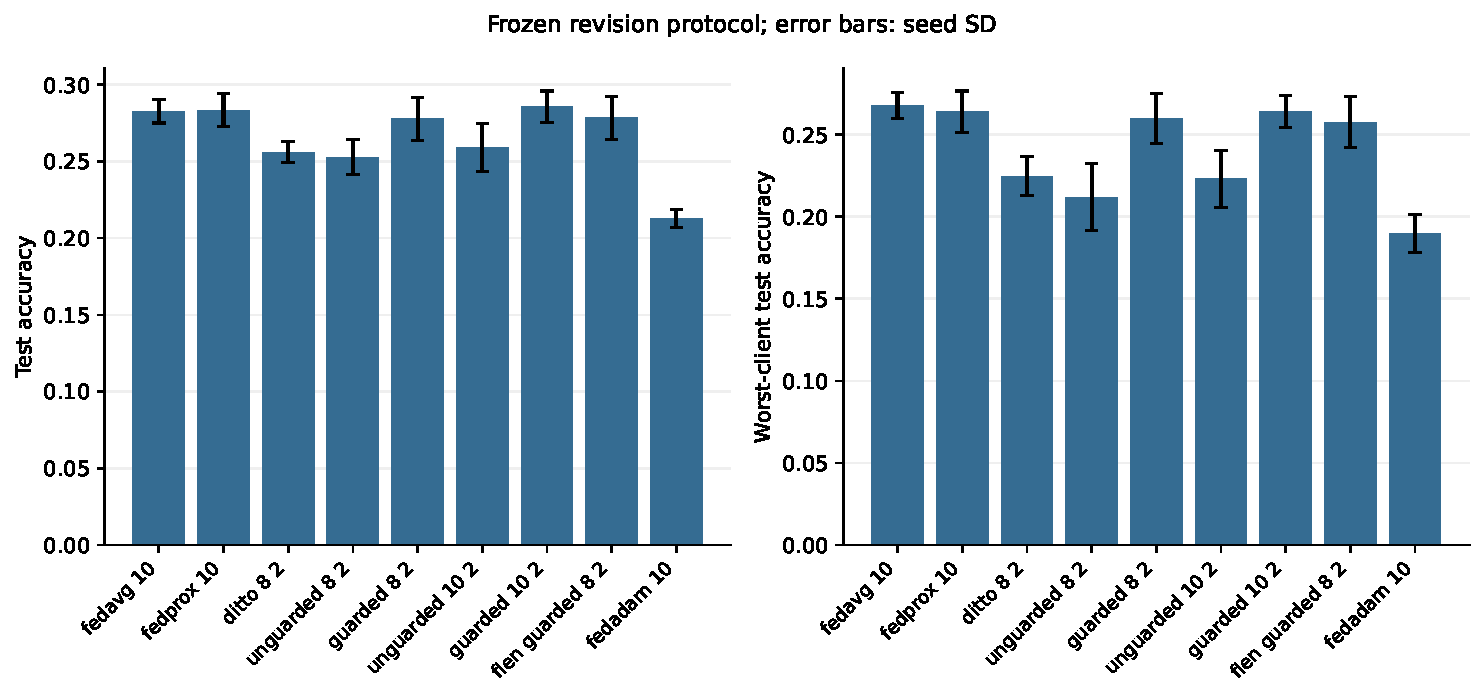
\includegraphics[width=\linewidth]{revision_casehold.pdf}
\caption{Completed dual-branch revision. Bars show five-seed means and seed SD on fixed test records. Worst client denotes a fixed test shard.}
\label{fig:revision-casehold}
\end{figure}
